
Multiple testing problems are a staple of modern data-driven studies, where a large number of hypotheses are formulated and screened for their plausibility simultaneously.
This multiplicity of tests brings along a multitude of challenges, which have been studied extensively in recent years.
% in the literature of high-dimensional statistics.


We are motivated in particular by problems in high-dimensional variable screenings for categorical data. 
A prototypical example in genetics application is genome-wide association studies (GWAS), where a large number of categorical genetic factors are examined for their potential influence on the phenotypic traits.
These categorical covariate screening problems naturally give rise to the high-dimensional chi-square models, introduced through the language of GWAS next.

\subsection{Genome-wide association studies and the chi-square model}
\label{subsec:motivation-chisq}

Broadly speaking, GWAS aim to discover genetic variations that are linked to traits or diseases of interested, by testing for associations between the subjects' genetic compositions and their phenotypes. (A nice introduction to this topic can be found in \citet{bush2012genome}.)
In a typical GWAS with case-control design, a total of $n$ subjects are recruited,  consisting of $n_1$ subjects possessing a defined trait, and $n_2$ subjects without the trait to serve as controls.
The genetic compositions of the subjects are then examined for variations known as single-nucleotide polymorphisms (SNPs) at an array of $p$ genomic marker locations, and compared between the case and the control group.

Focusing on one specific genomic location, the counts of observed genotypes, if two variants are present, can be tabulated as follows.
\begin{center}
    \begin{tabular}{cccc}
    \hline
    & \multicolumn{2}{c}{Genotype} & \\
    \cline{2-3}
    \# Observations & Variant 1 & Variant 2 & Total by phenotype \\
    \hline
    Cases & $O_{11}$ & $O_{12}$ & $n_1$ \\
    Controls & $O_{21}$ & $O_{22}$ & $n_2$ \\
    \hline
    \end{tabular}
\end{center}
Researchers test for associations between the two factors using, for example, the Pearson Chi-square test with statistic
\begin{equation} \label{eq:chisq-statistic}
    x = \sum_{j=1}^2 \sum_{k=1}^2 \frac{(O_{jk} - E_{jk})^2}{E_{jk}},
\end{equation}
where $E_{jk}$'s are the expected number of observations in respective cells under the null, estimated empirically with $E_{jk} = (O_{j1}+O_{j2})(O_{1k}+O_{2k})/n$.
%E_{jk} = \Big(\sum_{l}O_{jl}\Big)\Big(\sum_{l}O_{lk}\Big)\Big/n.

Under the mild assumption that the counts $O_{jk}$'s follow a multinomial distribution (or two independent binomial distributions), the statistic $x$ in \eqref{eq:chisq-statistic} can be shown to have an approximate $\chi^2(\lambda)$ distribution with $\nu=1$ degree of freedom at large sample sizes \citep{agresti2018introduction}. 
Independence between the genotypes and phenotypes would imply a non-centrality parameter $\lambda$ value of zero; if dependence exists, we have $\lambda\neq0$ where its value depends on the underlying multinomial probabilities.
More generally, if we have a $J$ phenotypes and $K$ genetic variants, assuming a $J\times K$ multinomial distribution, the statistic will follow approximately a $\chi^2_{\nu}(\lambda)$ distribution with $\nu = (J-1)(K-1)$ degrees of freedom, when sample sizes are large.

The same asymptotic distributional approximations are also apply to the likelihood ratio statistic, and many other statistics under slightly different modeling assumptions \cite{gao2019upass}.
These association tests are performed at each of the $p$ SNP marker locations throughout the whole genome, yielding $p$ statistics having approximately (non-)central $\chi^2_{\nu}$ distributions,
\begin{equation} \label{eq:model-chisquare-approx}
    x(i) \mathrel{\dot\sim} \chi_{\nu(i)}^2\left(\lambda(i)\right), \quad i=1,\ldots,p,
\end{equation}
where $\lambda = (\lambda(i))_{i=1}^p$ is the $p$-dimensional non-centrality parameter.
%, with $\lambda(i)=0$ indicating independence of the $i$-th SNP with the outcomes, and $\lambda(i)\neq0$ indicating associations.

Although the number of genomic locations $p$ can be in the order of $10^5$ or even $10^6$, it is often believed that only a small set of genetic variants have large influences on the outcome of the disease or trait of interest.
Under the stylized assumption of sparsity, $\lambda$ is assumed to have $s$ non-zero components, with $s$ being much smaller than the problem dimension $p$. 
The goal of researchers is two-fold: 1) to test if $\lambda(i)=0$ for all $i$, and 2) to estimate the set $S=\{i:\lambda(i)\neq 0\}$.
In other words, we look to first determine if there are \emph{any} genetic variations associated with the disease; if there are associations, we want to find their locations.

The latter, referred to as the \emph{support recovery problem}, is the focus of this work.
We will study in detail the theoretical limits of the support recovery problem in an idealized model where the statistics follow independent chi-square distributions,
\begin{equation} \label{eq:model-chisq}
    %x(i) \distras{\mathrm{ind.}} \chi_\nu^2\left(\lambda(i)\right), \quad i=1,\ldots,p.
    x(i) \sim \chi_\nu^2\left(\lambda(i)\right), \quad i=1,\ldots,p.
\end{equation}
We will also look for practical procedures that attain these performance limits, as soon as the problems become theoretically feasible.


\subsection{One-sided vs two-sided alternatives in additive error models}
\label{subsec:motivation-additive}

The chi-square model \eqref{eq:model-chisq} plays an important role in analyzing variable screening problems under omnidirectional alternatives.
A primary example is multiple testing under two-sided alternatives in the additive error model,
\begin{equation} \label{eq:model-additive}
    x(i) = \mu(i) + \epsilon(i), \quad i=1,\ldots,p,
\end{equation}
where the errors $\epsilon$ are assumed to have standard normal distributions.

Under two-sided alternatives, unbiased test procedures call for rejecting the hypothesis $\mu(i)=0$ at locations where observations have large absolute values, or equivalently, large squared values.
Squaring on both sides of \eqref{eq:model-additive}, we arrive at Model \eqref{eq:model-chisq} with non-centrality parameters $\lambda(i) = \mu^2(i)$, and degrees-of-freedom parameter $\nu =1$.
In this case, the support recovery problem is equivalent to locating the set of observations with mean shifts, $S=\{i:\mu(i)\neq 0\}$, where the mean shifts could take place in both directions.

While theoretical limits in the additive error model \eqref{eq:model-additive} have been recently studied in several papers, the asymptotic analyses therein focused either exclusively on the one-sided alternatives \cite{arias2017distribution, gao2018fundamental}, or exclusively on the two-sided alternatives \cite{butucea2018variable}.
Explicit comparisons between the two types of alternatives were not drawn, due in part to slightly different goals of these projects. We look to bridge this small gap in the current paper. 
In particular, we develop theories for both the two-sided alternatives (via the chi-square model \eqref{eq:model-chisq}) and the one-sided alternatives.
In comparing the results of these two cases, we will be able quantify if, and how much of a price has to be paid for the additional uncertainty in the two-sided alternatives versus the one-sided ones.

% In many applications, of course, restricting ourselves to one-sided tests is unrealistic.
% For example, in fMRI studies, the interest is in \emph{both} regions where average brain activities {increase} and where they {decrease}, when comparing the case group to the controls \citep{narayan2015two}. 
% In the challenging application of anomaly detection on Internet traffic streams, millions of IP addresses need to be scanned in real time to identify \emph{both} volumetric attacks and blackouts \citep{kallitsis2016amon}.
% Indeed, omnidirectional tests are the more natural choice in so-called discovery sciences where little to no prior knowledge is available.

\subsection{Asymmetric statistical risks}
\label{subsec:asymmetric-risk}

Another overlooked issue of practical importance is the choice of statistical risks.
In all aforementioned papers, the criteria for false discovery and non-discovery in support recovery problems are roughly \emph{symmetric}.
Specifically, \citet{arias2017distribution} studied conditions under which \emph{fractions} of false discovery and non-discovery can vanish; \citet{gao2018fundamental} investigated \emph{family-wise error control} for both types of errors; meanwhile, \citet{butucea2018variable} analyzed the problem under the Hamming loss, which penalizes false discoveries and missed detections \emph{equally}.

In applications, however, attitude towards type I and type II errors are often different.
In the example of GWAS, where the number of candidate locations $p$ could be in the millions, researchers are typically interested in the marginal (location-wise) power of discovery, while exercising stringent (family-wise) false discovery control --- a consideration not covered by existing theory.
Our observation on this asymmetry leads us to study, and discover, two new phase-transitions, both in the additive error model \eqref{eq:model-additive} under one-sided alternatives, and in the chi-square model \eqref{eq:model-chisq}.
The latter, as discussed in Section \ref{subsec:motivation-additive}, entails the additive error model \eqref{eq:model-additive} under two-sided alternatives.
% Further details can be found in Section \ref{subsec:risks} below, after 
% We summarize the main messages of this paper next.

\subsection{Contributions}

Our contribution is three-fold: (1) a thorough study of the theoretical limits of thresholding procedures in the chi-square model \eqref{eq:model-chisq} and the Gaussian additive error model \eqref{eq:model-additive}, (2) an enumeration of practical procedures attaining these limits, and (3) an illustration of the phase transition phenomena in genetic association studies.

We show that several commonly used family-wise error rate-control procedures --- including Bonferroni's procedure \cite{dunn1961multiple} --- are asymptotically optimal for the \emph{exact}, and \emph{exact-approximate} support recovery problems (defined in Section \ref{subsec:risks} below) in the chi-square model \eqref{eq:model-chisq}.
We further show that the Benjamini-Hochberg (BH) procedure \cite{benjamini1995controlling} is asymptotically optimal for the \emph{approximate}, and \emph{approximate-exact} support recovery problems (defined, too, in Section \ref{subsec:risks}).
These four results are made precise in Theorems \ref{thm:chi-squared-exact-boundary}, \ref{thm:chi-squared-exact-approx-boundary}, \ref{thm:chi-squared-approx-boundary}, and \ref{thm:chi-squared-approx-exact-boundary}.
Under appropriate parametrizations of the signal sizes and sparsity, they establish the phase transitions of support recovery problems in the chi-square model, previewed in Figure \ref{fig:phase-chi-squared}.
Remarkably, the degree-of-freedom parameter does not affect the asymptotic boundaries in any of the four support recovery problems.

In the same vein, we study the additive Gaussian error model \eqref{eq:model-additive} under \emph{one-sided alternatives}. 
% While phase transitions for the approximate and exact support recovery problems were discovered in \cite{arias2017distribution} and \cite{gao2018fundamental}, 
Two new results for the exact-approximate and approximate-exact support recovery problems are established here.
All phase transition boundaries (under suitable parametrizations) coincide with those in the chi-square models.
% and Figure \ref{fig:phase-chi-squared} continues to apply.
Following the discussion in Section \ref{subsec:motivation-additive}, this indicates vanishing differences between the difficulties of the one-sided and two-sided alternatives in the additive error model \eqref{eq:model-additive}.

%The many interesting results obtained under one-sided alternatives cannot be easily adapted to the two-sided cases where the locations and the directions of the signals are both unknown.

Finally, we return to association screenings of categorical variables, and 
present empirical evidence for the phase transition in the exact-approximate problem using real data from large-scale association studies on breast cancer obtained from the NHGRI-EBI GWAS Catalog \cite{macarthur2016new}.
% demystify the notion of signal size $\lambda$ in this context.
% which is perhaps less transparent than in additive error models.
We do so by characterizing of the relationship between the signal size $\lambda$ and the marginal frequencies, odds ratio, and sample sizes for association tests on 2-by-2 contingency tables.
% Specifically, the amount of signal, when rare variants are present, is weaker compared to the signal when the marginal distributions are balanced.
% In other words, reliable detection of the effects by rare variants would require more samples compared to common variants, even at the same odds ratio.
This result, establishing the relationship between sample sizes and signal sizes, is made precise in Proposition \ref{prop:signal-size-odds-ratio}.
Of independent interest, a corollary of the proposition also enables us to determine the optimal design for association studies under a fixed budget, and reveals that balanced designs with equal number of cases and controls are often statistically inefficient.

We illustrate practical use of these results in power analysis with numerical examples. Results on phase transitions are demonstrated with simulations in Section \ref{sec:numerical}.

% Practical issues are also addressed to make for simple and effective power analysis.

\subsection{Statistical risks in support recovery problems}
\label{subsec:risks}

\begin{figure}
      \centering
      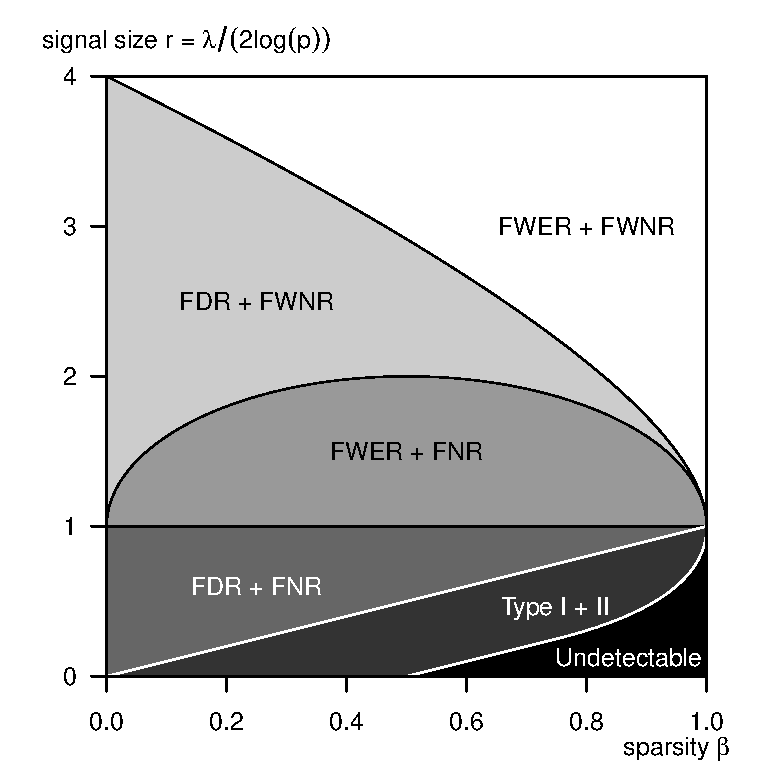
\includegraphics[width=0.6\textwidth]{./phase_diagram_chisquared_ALL_boundaries.eps}
      % 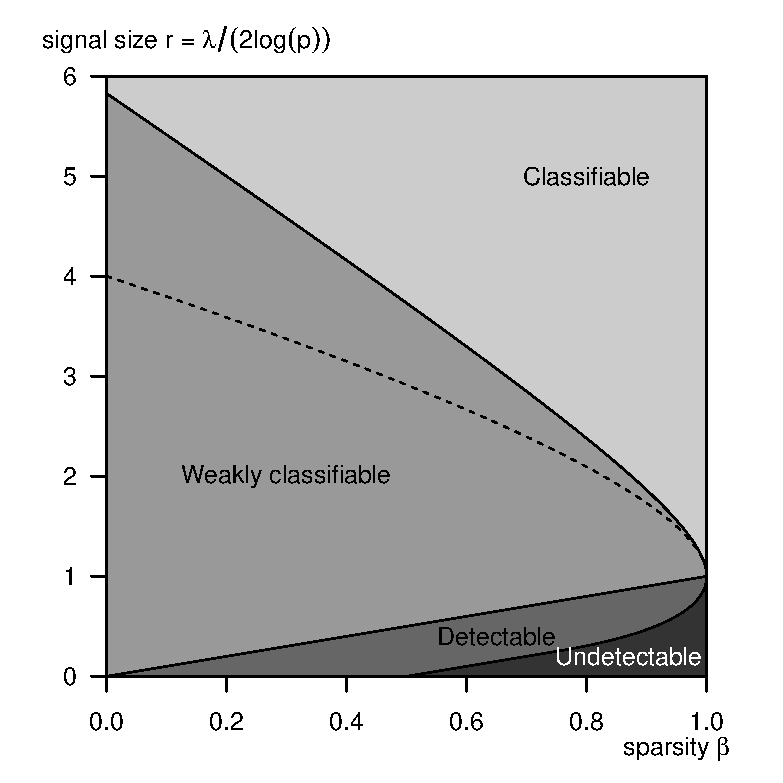
\includegraphics[width=0.35\textwidth]{./phase_diagram_chisquared.eps}
      \caption{The phase diagram for sparse problems in the high-dimensional chi-square model \eqref{eq:model-chisq}, illustrating the boundaries of the exact support recovery (FWER + FWNR; top curve; Theorem \ref{thm:chi-squared-exact-boundary}),
      the exact-approximate support recovery (FDR + FWNR; second curve; Theorem \ref{thm:chi-squared-exact-approx-boundary}),
      the approximate-exact support recovery (FWER + FNR; horizontal line $r=1$; Theorem \ref{thm:chi-squared-approx-exact-boundary}),
      and the approximate support recovery (FDR + FNR; tilted line $r=\beta$; Theorem \ref{thm:chi-squared-approx-boundary}) problems.
      The signal detection problem (type I + type II errors of the global test; lower curve) was studied in \citep{donoho2004higher}. 
      In each region of the diagram and above, the marked statistical risk can be made to vanish, as dimension $p$ diverges. 
      Conversely, the risks has liminf at least one.
      All boundaries are unaffected by the degrees-of-freedom.
      All boundaries are identical to those in the Gaussian additive error model \eqref{eq:model-additive} under one-side alternatives, setting $\lambda=\mu^2$.} 
      \label{fig:phase-chi-squared}
\end{figure}

Recall that in support recovery problems, our goal is to come up with a procedure, denoted $\mathcal R$, to produce a set estimate $\widehat{S}$ of the true index set of relevant variables  $S=\{i:\lambda(i)\neq 0\}$.
The set estimate depends on the procedure $\mathcal{R}$, which in turn, takes as input the data or test statistics $x$.
We suppress this dependence by writing $\widehat{S}$ in place of $\widehat{S}(\mathcal{R}(x))$ for notational convenience when it does not lead to ambiguity.

For a given procedure $\mathcal{R}$, the \emph{false discovery rate} (FDR) of the procedure is defined to be the expected fraction of false findings not in the true index set, among the reported discoveries \cite{benjamini1995controlling}. 
Its counterpart, \emph{false non-discovery rate} (FNR), measuring the power of the procedure, is defined as the expected fraction of missed detection. 
Mathematically, we define
\begin{equation} \label{eq:FDR-FNR}
    \mathrm{FDR}(\mathcal{R}) = \E\left[\frac{|\widehat{S}\setminus S|}{\max\{|\widehat{S}|,1\}}\right],
    \quad \text{and} \quad
    \mathrm{FNR}(\mathcal{R}) = \E\left[\frac{|S\setminus \widehat{S}|}{\max\{|{S}|,1\}}\right],
\end{equation}
where the maxima in the denominators resolve the otherwise division by 0 problem. 
Roughly speaking, the FNR describes the proportion of type II errors among the true signals, and reflects marginal power of the procedure.

A more stringent criteria for false discovery in multiple testing problems is family-wise error rate (FWER), defined to be the probability of reporting at least one finding not contained in the true index set.
Correspondingly, a more stringent criteria for false non-discovery is family-wise non-discovery rate (FWNR), defined as the probability of missing at least one signal in the true index set. That is,
\begin{equation} \label{eq:FWER-FWNR}
    \mathrm{FWER}(\mathcal{R}) = 1 - \P[\widehat{S} \subseteq S], 
    \quad \text{and} \quad
    \mathrm{FWNR}(\mathcal{R}) = 1 - \P[S \subseteq \widehat{S}].
\end{equation}

We introduce four different ways to quantified statistical risks in support recovery problems, leading to different inferential limits. 
Following \cite{arias2017distribution}, we define the risk for \emph{approximate} support recovery as
\begin{equation} \label{eq:risk-approximate}
    \mathrm{risk}^{\mathrm{A}}(\mathcal{R}) = \mathrm{FDR}(\mathcal{R}) + \mathrm{FNR}(\mathcal{R}).
\end{equation}
Analogously, we define the risk for \emph{exact} support recovery as
\begin{equation} \label{eq:risk-exact}
    \mathrm{risk}^{\mathrm{E}}(\mathcal{R}) = \mathrm{FWER}(\mathcal{R}) + \mathrm{FWNR}(\mathcal{R}).
\end{equation}
An intimately related measure of success in the exact support recovery risk is the probability of exact recovery, 
\begin{equation} \label{eq:risk-prob}
    \P[\widehat{S} = S] = 1 - \P[\widehat{S} \neq S].
\end{equation}
The relationship between $\P[\widehat{S} = S]$ and $\mathrm{risk}^{\mathrm{E}}$ will be analyzed in Section \ref{sec:chisq-boundaries}.

The discussion in Section \ref{subsec:asymmetric-risk} --- and in particular, the GWAS application --- prompts us to consider risks that reflect both the family-wise error rate and the marginal power of discovery.
One such risk metric is what we call the \emph{exact-approximate} support recovery risk
\begin{equation} \label{eq:risk-exact-approx}
    \mathrm{risk}^{\mathrm{EA}}(\mathcal{R}) = \mathrm{FWER}(\mathcal{R}) + \mathrm{FNR}(\mathcal{R}).
\end{equation}
Analogously, we consider the \emph{approximate-exact} support recovery risk
\begin{equation} \label{eq:risk-approx-exact}
    \mathrm{risk}^{\mathrm{AE}}(\mathcal{R}) = \mathrm{FDR}(\mathcal{R}) + \mathrm{FWNR}(\mathcal{R}),
\end{equation}
which places more emphasis on non-discovery control.
% These two risks differ in their stringency in controlling false discovery and false non-discovery.
Theoretical limits and performance of procedures in support recovery problems will be studied in terms of the five risk metrics \eqref{eq:risk-approximate}, \eqref{eq:risk-exact}, \eqref{eq:risk-prob}, \eqref{eq:risk-exact-approx} and \eqref{eq:risk-approx-exact}, defined above.

\subsection{Thresholding procedures}
\label{subsec:thresholding-procedures}

We shall study the performance of five procedures in Section \ref{sec:chisq-boundaries}.
All of them belong to the broad class of thresholding procedures, defined as follows.
\begin{definition}[Thresholding procedures]
A thresholding procedure for estimating the support 
$S:=\{i\, :\, \lambda(i)\neq0\}$ is one that takes on the form
\begin{equation} \label{eq:thresholding-procedure}
    \widehat{S} = \left\{i\,|\,x(i) \ge t(x)\right\},
\end{equation}
where the threshold $t(x)$ may depend on the data $x$.
\end{definition}
Examples of thresholding procedures include ones that aim to control FWER -- Bonferroni's \cite{dunn1961multiple}, Sid\'ak's \citep{vsidak1967rectangular}, Holm's \citep{holm1979simple}, and Hochberg's procedure \citep{hochberg1988sharper} -- as well as ones that target FDR, such as Benjamini-Hochberg's procedure \cite{benjamini1995controlling} and Cand\'es-Barber's procedure \cite{barber2015controlling}.
Indeed, thresholding procedures \eqref{eq:thresholding-procedure} is such a general class that it contains most of the statistical procedures in the multiple testing literature \cite{roquain2011type}.

We shall restrict our discussion to the class of thresholding procedures.
Specifically, the lower bounds that we develop in Theorems \ref{thm:chi-squared-exact-boundary} through \ref{thm:chi-squared-approx-exact-boundary} below are only meant to apply to such procedures.

\begin{remark}
Although it is intuitively appealing to consider only threshold procedures, such procedures are not always optimal.
Recently, \citet{chen2018scan} showed that thresholding procedures are in fact sub-optimal in the additive models \eqref{eq:model-additive} when errors have heavy (regularly-varying) tails. 
\citet{gao2018fundamental} recently characterized the conditions under which thresholding procedures are optimal in the exact support recovery problems.
The optimality of thresholding procedures in terms other statistical risks is an open problem that invites a dedicated discussion in a future study. 
% We content ourselves with making optimality statements concerning only thresholding procedures in the current work.
\end{remark}


\subsection{More related work}

Performance limits of statistical procedures in the additive error model \eqref{eq:model-additive} have been actively studied in recent years.
Specifically, when the approximate support recovery risk \eqref{eq:risk-approximate} is used as the criterion, the asymptotic optimality of the Benjamini-Hochberg procedure \cite{benjamini1995controlling}, and the Cand\'es-Barber procedure \cite{barber2015controlling} was established by \citet*{arias2017distribution} under independent additive errors and one-sided alternatives.
% \citet{rabinovich2017optimal} further established the rate-optimality of both procedures under the same regime.

In terms of the more stringent exact support recovery probability \eqref{eq:risk-prob}, several well-known FWER-controlling procedures --- including Bonferroni's procedure --- have been shown to be optimal in the additive error model under one-sided alternatives. This is so, even under severe dependence and general distributional assumptions \cite{gao2018fundamental}.
Interesting optimality results were also obtained for a specific procedure under the expected Hamming loss, $\E[\widehat{S}\triangle S]$, in the additive model when errors are Gaussian \cite{butucea2018variable}.

There is a wealth of literature on the so-called sparsistency (i.e., $\P[\widehat{S} = S]\to 1$ as $p\to\infty$) problem in the regression context. 
We refer readers to the recent book by \citet{wainwright2019high} (and in particular, the bibliographical sections of Chapters 7 and 15) for a comprehensive review.
We only mention two additional papers by \citet{ji2012ups} and \citet{jin2014optimality} which derived minimax optimality results under the Hamming loss in this context.

The asymptotic optimality of the Bonferroni and BH procedures 
% in the Gaussian scale mixture model 
was analyzed under decision theoretic frameworks in \cite{genovese2002operating, bogdan2011asymptotic, neuvial2012false}, with main focus on location/scale models. In particular, these papers show that the statistical risks of the practical procedures approach that of the oracle procedures in suitable asymptotic regimes.
Strategies for dealing with multiple testing under general distributional assumptions can be found in, e.g., \cite{efron2004large, storey2007optimal, sun2007oracle}, where the non-nulls are assumed to follow a common distribution; the two-sided alternative in the additive error model was featured as the primary example in \cite{sun2007oracle}.
Although weighted sums of false discovery and non-discovery have been studied in the literature, asymmetric statistical risks such as \eqref{eq:risk-exact-approx} and \eqref{eq:risk-approx-exact} are new.
The high-dimensional chi-square model \eqref{eq:model-chisq} also seemed to have received little attention.
While the sparse signal detection problem in the chi-square model has been studied \cite{donoho2004higher}, support recovery problems, to the best of our knowledge, remain unexplored.
% In particular, \citet{sun2007oracle} studied likelihood thresholding procedure % ; their proposed likelihood ratio thresholding procedure requires consistent estimation of the non-null distributions and the mixture proportions.

Finally, asymptotic power approximations of association tests on contingency tables can be found in, e.g., \citet{ferguson2017course}, or other texts on asymptotic statistics.
A companion paper to the current work analyzes asymptotic equivalences of several additional common association tests, and implements second order power approximations in a software tool \cite{gao2019upass}. 
The software also facilitates visualization and forensics of reported findings in genetic association studies.


